\documentclass{article}
\usepackage{geometry}
\usepackage{amsmath}
\usepackage{amsfonts}
\usepackage{amssymb}
\usepackage{amsthm}
\usepackage{parskip}
\usepackage{multicol}
\usepackage{xcolor}
\usepackage{fancyhdr}
\usepackage{physics}
\usepackage{graphicx} % Required for inserting images
\usepackage{hyperref}
\usepackage{enumitem}
\usepackage{mathtools}

% commands
\newcommand{\deq}{\vcentcolon=}
\newcommand{\idd}{\text{đ}}
\newcommand{\nimplies}{\centernot\implies}
\newcommand{\vc}[1]{\boldsymbol{#1}}

% margin settings
\geometry{
    a4paper,
    left=7mm,
    right=7mm,
    top=2cm,
    bottom=7mm
}

% testing
\usepackage{blindtext}

% proof environments
\newtheorem{definition}{Definition}[section]
\newtheorem{theorem}{Theorem}[section]
\newtheorem{corollary}{Corollary}[theorem]
\newtheorem{lemma}[theorem]{Lemma}
\newtheorem*{remark}{Remark} % unnumbered remarks

% header and footer
\pagestyle{fancy}
\fancyfoot{} % removes footer
\fancyhf{}
\renewcommand{\headrulewidth}{0.5pt}
\fancyhead[L]{Honours complex variables}
\fancyhead[R]{\thepage}

\begin{document}

\begin{multicols*}{3}
% starred environment ensures text remains in same column
\noindent

\subsubsection*{D1.1.1: Complex numbers}
Let $z=x+iy$ and $w=a+ib$ where $x,y,a,b\in\mathbb{R}$.
Then $z$ and $w$ are complex numbers. Furthermore:
\begin{enumerate}
    \item $z=w$ \textbf{if{}f} $x=a$ and $y=b$.
    
    \item $\Re(z)\deq x$ and $\Im(z)\deq y$.
    
    \item $|z|\deq\sqrt{x^2+y^2}$
    
    \item The \textbf{complex conjugate} of $z$ is:
    $$z^*\deq x-iy.$$

    \item Addition and multiplication:
    $$(x+iy)+(a+ib)=(x+a)+i(y+b)$$
    $$(x+iy)(a+ib)=(xa-yb)+i(xb+ya).$$

    \item $\mathbb{C}\deq\{x+iy:x,y\in\mathbb{R}\}$
\end{enumerate}
with rule $i^2=-1$.

\subsubsection*{L1.1.3}
Let $u,w,z\in\mathbb{C}$ where $z=x+iy$. Then:
\begin{enumerate}
    \item $z+w=w+z$ and $zw=wz$.
    
    \item $u+(z+w)=(u+z)+w$
    
    \item $u(zw)=(uz)w$
    
    \item $u(z+w)=uz+uw$
    
    \item $z+0=z$ and $1z=z$.
    
    \item $\exists\bigl(-z\deq-x+i(-y)\bigr)$:
    $z+(-z)=0$.

    \item $\exists z^{-1}: zz^{-1}=1$ where:
    $$z^{-1}\deq\frac{x}{x^2+y^2}+i\frac{-y}{x^2+y^2}.$$
\end{enumerate}

\subsubsection*{D1.1.5 and D1.1.7: Polar form}
Let $z\in\mathbb{C}$ and $z=x+iy$. Then:
\begin{align*}
    z
    &=r(\cos\theta+i\sin\theta) \\
    &=re^{i\theta}
\end{align*}
for $\textcolor{red}{r=|z|}=\sqrt{x^2+y^2}$ and
$\theta\in(-\pi,\pi]$ is given by $\tan\theta=y/x$.
\begin{center}
    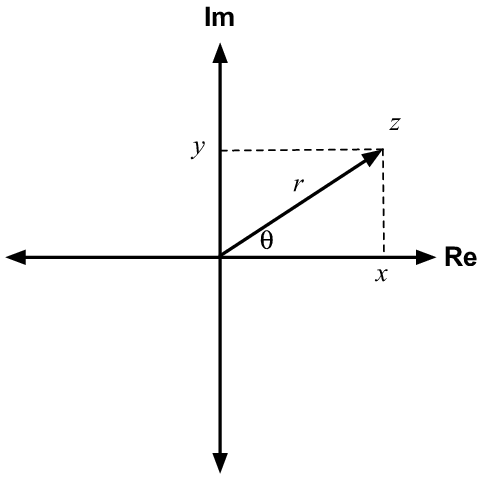
\includegraphics[scale=0.2]{f0.png}
\end{center}

\subsubsection*{L1.1.6}
Let $\theta,\phi\in\mathbb{R}$ and $n\in\mathbb{Z}$. Then:
\begin{enumerate}
    \item $e^{i(\theta+\phi)}=e^{i\theta}e^{i\phi}$
    
    \item $e^{in\theta}=(e^{i\theta})^n$
\end{enumerate}
due to de Moivre's formula:
$$\cos n\theta+i\sin n\theta=(\cos \theta+i\sin \theta)^n.$$

\newcolumn

\subsubsection*{L1.1.9}
Let $z,w\in\mathbb{C}$. Then:
\begin{enumerate}
    \item $|z|=0$ \textbf{if{}f} $z=0$.
    
    \item $|\overline{z}|=|z|$
    
    \item $|zw|=|z||w|$
    
    \item $(z^*)^*=z$
    
    \item $|z|^2=zz^*$ and $|z^2|=|z|^2$.
    
    \item $(z+w)^*=z^*+w^*$
    
    \item $(zw)^*=z^*\hspace{0.01in}w^*$
    
    \item $|\Re(z)|\leq|z|$ and $|\Im(z)|\leq|z|$.
    
    \item $\Re(z)=\frac{1}{2}(z+z^*)$
    
    \item $\Im(z)=\frac{1}{2i}(z-z^*)$.
\end{enumerate}

\subsubsection*{L1.1.10 -- 11: Triangle inequalities}
Let $z,w\in\mathbb{C}$. Then:
\begin{enumerate}
    \item $|z+w|\leq|z|+|w|$
    
    \item $||z|-|w||\leq|z-w|$.
\end{enumerate}

\subsubsection*{D1.1.12: Argument of $z$}
The set of all arguments of $z$ is:
\begin{align*}
    \arg(z)
    &\deq\{\theta:z=|z|e^{i\theta}\} \\
    &=\{\text{Arg}(z)+2\pi k:k\in\mathbb{Z}\}.
\end{align*}
The \textcolor{red}
{principle argument of $z$} satisfies \\
$z=|z|e^{i\text{Arg}(z)}$ with
$-\pi<\text{Arg}(z)\leq\pi$.
$$\therefore\text{Arg}(z)\equiv\arg(z)\mod 2\pi$$
$\text{Arg}(z)$ is discontinuous on the negative real axis
since $\forall x,\epsilon>0;-x\pm i\epsilon\rightarrow x$:
$$\lim_{\epsilon\rightarrow0}\text{Arg}(-x\pm i\epsilon)=\pm\pi.$$

\subsubsection*{P1.1.14}
Let $z,w\in\mathbb{C}$. Then:
\begin{enumerate}
    \item $\arg(zw)=\arg(z)+\arg(w)$
    
    \item $\arg(z^*)=-\arg(z)$
\end{enumerate}
for these are set operations.

\subsubsection*{D1.2.1: Open and closed $\epsilon$-discs}
Let $z_0\in\mathbb{C}$ and $\epsilon>0$.
\begin{enumerate}
    \item An \textbf{open} $\epsilon$-disc
    centred at $z_0$ is:
    $$D_{\epsilon}(z_0)
    \deq\{z\in\mathbb{C}:|z-z_0|<\epsilon\}.$$

    \item A \textbf{closed} $\epsilon$-disc
    centred at $z_0$ is:
    $$\overline{D}_{\epsilon}(z_0)
    \deq\{z\in\mathbb{C}:|z-z_0|\leq\epsilon\}.$$
\end{enumerate}
A \textbf{punctured} $\epsilon$-disc centred at $z_0$ is:
$$D'_{\epsilon}(z_0)\deq\{z\in\mathbb{C}:0<|z-z_0|<\epsilon\}.$$

\subsubsection*{D1.2.2: Open and closed sets}
Let $U\subset\mathbb{C}$. Set $U$ is \textbf{open} if:
$$\forall z_0\in U;\exists\epsilon>0:D_{\epsilon}(z_0)\subseteq U.$$
Subset $F$ is \textbf{closed} if
$\mathbb{C}\hspace{0.02in}\backslash\hspace{0.02in} F$ is open.

A \textbf{neighbourhood} of point $z_0\in\mathbb{C}$
is an open set that contains $z_0$.

\subsubsection*{Remark}
$\emptyset$ is \textcolor{red}{vacuously} open.
Therefore $\mathbb{C}$
is open \textbf{and} closed.
A set
like $D_2(0)\hspace{0.01in}\backslash\hspace{0.01in}
D_1(0)$
is \textbf{neither closed nor open}.

The union and intersection of open sets is
also an open set.

\subsubsection*{L1.2.3}
Punctured disc $D'_{\epsilon}(z_0)$ is open.

\subsubsection*{D1.2.4: Limit points}
Let $S\subseteq\mathbb{C}$. $z_0$ is a \textbf{limit point} of $S$ if:
$$\forall\epsilon>0; D'_{\epsilon}(z_0)\cap S\neq\emptyset.$$
The \textbf{closure} of $S$ is set $\overline{S}$ and contains $S$
and \textbf{all} its limit points.

\subsubsection*{L1.2.6}
Let $S\subseteq\mathbb{C}$.
$S$ is closed \textbf{if{}f} $S=\overline{S}$.

\subsubsection*{D1.2.7: Bounded sets}
Let $S\subseteq\mathbb{C}$. Set $S$ is \textbf{bounded} if:
$$\forall z\in S;\exists M>0:|z|\leq S.$$

\subsubsection*{D1.2.8: $\epsilon$-N convergence}
Let $\mathbb{N}=\{0,1,2,\dots\}$.

Let $(z_n)_{n\in\mathbb{N}}\subseteq\mathbb{C}$ be a sequence
and $z\in\mathbb{C}$.
Then $\displaystyle\lim_{n\rightarrow\infty}z_n=z$ if:
\begin{align*}
    &\forall\epsilon>0;\exists N\in\mathbb{N}:\forall n\geq N \\
    &\implies |z_n-z|<\epsilon.
\end{align*}

\subsubsection*{L1.2.9}
Let $z_n,z\in\mathbb{C}$ where $z_n=a_n+i b_n$.

Then $\displaystyle\lim_{n\rightarrow\infty}z_n=z$ \textbf{if{}f}:
$$\Re(z)=\lim_{n\rightarrow\infty}a_n
\hspace{0.05in}\text{and}\hspace{0.05in}
\Im(z)=\lim_{n\rightarrow\infty}b_n.$$

\subsubsection*{L1.2.10}
Let $S\subseteq\mathbb{C}$ and $z\in\mathbb{C}$.
Then $z\in\overline{S}$ \textbf{if{}f}:
$$\exists z_n\in S: z=\lim_{n\rightarrow\infty}z_n.$$

\subsubsection*{D1.2.11: Cauchy sequences}
$z_n$ is a Cauchy sequence if:
\begin{align*}
    &\forall\epsilon>0;\exists N\in\mathbb{N}:
    \forall n,m\geq N \\
    &\implies |z_n-z_m|<\epsilon.
\end{align*}

\subsubsection*{L1.2.12}
$z_n$ is convergent \textbf{if{}f} $z_n$ is Cauchy.

\subsubsection*{D1.2.14: Bounded sequences}
$z_n$ is bounded if:
$$\forall n\in\mathbb{N};\exists M>0:|z_n|\leq M.$$

\subsubsection*{L1.2.15: Bolzano-Weierstrass}
Let $z_n$ be a bounded sequence. Then:
$$\exists (z_{n_k})_{k,n_k\in\mathbb{N}}:
\lim_{k\rightarrow\infty}z_{n_k}=z\in\mathbb{C}$$
or that $z_n$ has a convergent subsequence.

A selection of a sequence is a subsequence.

\subsubsection*{D1.3.1: Bounded functions}
Let $S\subseteq\mathbb{C}$ and $f:S\rightarrow\mathbb{C}$.
Then $f$ is a bounded function if:
$$\forall z\in S;\exists M>0:|f(z)|\leq M.$$

\subsubsection*{D1.3.2: $\epsilon$-$\delta$ convergence}
Let $S\subseteq\mathbb{C}, z_0\in\overline{S},f:S\rightarrow\mathbb{C}$
and $a_0\in\mathbb{C}$.
Then $\displaystyle\lim_{z\rightarrow z_0}f(z)=a_0$ if:
\begin{align*}
    &\forall z\in S;\forall\epsilon>0;\exists\delta>0:
    0<|z-z_0|<\delta \\
    &\implies|f(z)-a_0|<\epsilon.
\end{align*}

\subsubsection*{L1.3.3}
Let $S\subseteq\mathbb{C}, z_0\in\overline{S},
f:S\rightarrow\mathbb{C}$ and $a_0\in\mathbb{C}$ where $z_0=x_0+iy_0$
and $f=u+iv$.

Then $\displaystyle\lim_{z\rightarrow z_0}f(z)=a_0$ \textbf{if{}f}:
$$\Re(a_0)=\lim\limits_{\substack{
    x \to x_0 \\
    y \to y_0}}u(x,y)$$
and
$$\Im(a_0)=\lim\limits_{\substack{
    x \to x_0 \\
    y \to y_0}}v(x,y).$$

\subsubsection*{L1.3.4}
Let $S\subseteq\mathbb{C}, z_0\in\overline{S},
f:S\rightarrow\mathbb{C},a_0\in\mathbb{C}$ and sequence
$w_n\in S\hspace{0.02in}\backslash\hspace{0.02in}\{z_0\}$.

If $\displaystyle\lim_{z\rightarrow z_0}f(z)=a_0$
and $\displaystyle\lim_{n\rightarrow\infty}w_n=z_0$
then:
$$\lim_{n\rightarrow\infty}f(w_n)=a_0.$$

\subsubsection*{L1.3.5: Limit identities}
Let $S\subseteq\mathbb{C}, z_0\in\overline{S}$ and $a_0,b_0\in\mathbb{C}$. \\
Let $f,g:S\rightarrow\mathbb{C}$.

If $\displaystyle\lim_{z\rightarrow z_0}f(z)=a_0$
and $\displaystyle\lim_{z\rightarrow z_0}g(z)=b_0$
then:
\begin{enumerate}
    \item $\displaystyle\lim_{z\rightarrow z_0}
    (f(z)+g(z))=a_0+b_0$

    \item $\displaystyle\lim_{z\rightarrow z_0}
    (f(z)g(z))=a_0 b_0$

    \item $\displaystyle\lim_{z\rightarrow z_0}
    \left(\frac{f(z)}{g(z)}\right)=\frac{a_0}{b_0}$
    if $b_0\neq0$.
\end{enumerate}

\subsubsection*{D1.3.6: $\epsilon$-$\delta$ continuity}
Let $S\subseteq\mathbb{C}, f:S\rightarrow\mathbb{C}$
and $z_0\in S$.
Then $f$ is continuous at $z_0$ if:
\begin{align*}
    &\forall z\in S;\forall\epsilon>0;\exists\delta>0:
    |z-z_0|<\delta \\
    &\implies|f(z)-f(z_0)|<\epsilon.
\end{align*}

\subsubsection*{L1.3.7}
Let $f:\mathbb{C}\rightarrow\mathbb{C}$ with rule $f=u+iv$
and $z_0=x_0+iy_0\in\mathbb{C}$.

Then $f$ is continuous at $z_0$ \textbf{if{}f}
$u$ and $v$ are continuous at $(x_0,y_0)$.

\subsubsection*{L1.3.8}
If $f,g:\mathbb{C}\rightarrow\mathbb{C}$
are continuous at $z_0$ then:
\begin{enumerate}
    \item $f+g$ is continuous at $z_0$.
    
    \item $fg$ is continuous at $z_0$.
    
    \item $f/g$ is continuous at $z_0$.
    ($g\neq0$)
\end{enumerate}

\subsubsection*{D: Image and preimage}
Let $f:X\rightarrow Y$ where $A\subseteq X$ and $B\subseteq Y$.
The image of $A$ is:
$$f(A)=\{f(x):x\in A\}$$
and the preimage of $B$ is:
$$f^{-1}(B)=\{x:f(x)\in B\}.$$

\subsubsection*{L1.3.9}
Let $U\subseteq\mathbb{C}$ be an open set.
$f:\mathbb{C}\rightarrow\mathbb{C}$ is continuous \textbf{if{}f}
$\forall U\subseteq\mathbb{C}; f^{-1}(U)$ is open
for $f^{-1}(U)=\{z\in\mathbb{C}:f(z)\in U\}$.

\subsubsection*{L1.3.10}
Let $f:S\rightarrow\mathbb{C}$ be continuous.
Let $S\subseteq\mathbb{C}$ be closed and bounded.

Then $f(S)$ is closed and bounded.

\subsubsection*{D1.4.1: Differentiability}
Let $z_0\in\mathbb{C}$ and $U$ a neighbourhood of $z_0$.
Let $f:U\rightarrow\mathbb{C}$. Then $f$ is differentiable at $z_0$ if
the following limit exists:
$$f'(z_0)\deq\lim_{z\rightarrow z_0}\frac{f(z)-f(z_0)}{z-z_0}.$$

\subsubsection*{L1.4.3}
Differentiability $\implies$ continuity.

Let $z_0\in\mathbb{C}$ and $U$ a neighbourhood of $z_0$.
If $f:U\rightarrow\mathbb{C}$ is differentiable at $z_0$ then
$f$ is continuous at $z_0$.

\subsubsection*{L1.4.4}
Let $z_0\in\mathbb{C}$ and $U$ a neighbourhood of $z_0$.
Let $f,g:U\rightarrow\mathbb{C}$ be differentiable at $z_0$.
Then $f+g$, $fg$ and $f/g$ (where $g(z_0)\neq0$)
are all differentiable at $z_0$.

\subsubsection*{L1.4.5: Chain rule}
Let $z_0\in\mathbb{C}$ and $U$ a neighbourhood of $z_0$.
Let $g:U\rightarrow\mathbb{C}$ be such that $g(U)$ is a neighbourhood
of $g(z_0)$. Assume that $g$ is differentiable at $z_0$
and $f$ is differentiable at $g(z_0)$. Then $f\circ g$
is differentiable at $z_0$:
$$(f\circ g)'(z_0)=f(g(z_0))g'(z_0).$$

\subsubsection*{T1.4.6: Cauchy-Riemann equations}
Let $z_0\in\mathbb{C}$ and $U$ a neighbourhood of $z_0$.
Let $f:U\rightarrow\mathbb{C}$ be differentiable at $z_0$. \\
Let $z_0=x_0+i y_0$ and $f=u+iv$. Then:
$$\frac{\partial u}{\partial x}(x_0,y_0)
=\frac{\partial v}{\partial y}(x_0,y_0)$$
$$\frac{\partial u}{\partial y}(x_0,y_0)
=-\frac{\partial v}{\partial x}(x_0,y_0)$$
and are the Cauchy-Riemann equations.

\subsubsection*{T1.4.8}
Let $z_0\in\mathbb{C}$ and $U$ a neighbourhood of $z_0$
for $z_0=x_0+i y_0$. Let $f:U\rightarrow\mathbb{C}$ where $f=u+iv$.

Assume that $u$ and $v$ have
\textcolor{red}{continuous first derivatives}
on a neighbourhood of $(x_0,y_0)$ \textbf{and} also that they
\textcolor{red}{satisfy the Cauchy Riemann equations}
at $(x_0,y_0)$.

Then $f$ is differentiable at $z_0$.

\subsubsection*{D1.4.9: Holomorphic functions}
$f$ is \textbf{holomorphic} at $z_0$ if there exists a neighbourhood
$U$ of $z_0$ such that $f$ is defined and differentiable.

\subsubsection*{D1.4.13: Harmonic equations}
$h(x,y)$ is harmonic if for
$\forall(x,y)\in\mathbb{R}^2$ it satisfies Laplace's equation:
$$\frac{\partial^2h}{\partial x^2}(x,y)+
\frac{\partial^2h}{\partial y^2}(x,y)=0.$$

\subsubsection*{L1.4.14}
Let $u(x,y),v(x,y)$ be twice continuously differentiable
and that $f(x+iy)=u+iy$ is holomorphic on $\mathbb{C}$.

Then $u$ and $v$ are harmonic.

\subsubsection*{D1.4.15: Harmonic conjugates}
Let $U\subseteq\mathbb{R}^2$ and
$u:U\rightarrow\mathbb{R}$ be harmonic.
Then harmonic function $v:U\rightarrow\mathbb{R}$ is a
\textbf{harmonic conjugate} of $u$ if complex function
$f=u+iv$ is holomorphic on $U$.

\subsubsection*{D1.5.1: Polynomial degree}
Let $P:\mathbb{C}\rightarrow\mathbb{C}$ be a polynomial.
The \textbf{degree} of $P$ 
is the highest power of the variable in $P$,
denoted as $\deg(P)$.

\subsubsection*{L1.5.2}
Let $z_0\in\mathbb{C}$. Let complex functions $f$ and $g$ be
holomorphic at $z_0$. Then $f+g$, $fg$ and $f/g$ ($g\neq0$)
are holomorphic at $z_0$.

\subsubsection*{C1.5.3}
Let $N\in\mathbb{N}$ and $a_0,\dots,a_N\in\mathbb{C}$. \\
Let $\displaystyle P(z)=\sum_{n=0}^{N}a_n z^n$. \\
Then $P(z)$ is holomorphic on $\mathbb{C}$ and:
$$P'(z_0)=\sum_{n=1}^{N}na_n z_0^{n-1}.$$

\subsubsection*{L1.5.4}
Let $\displaystyle P(z)=\sum_{n=0}^{N}a_n z^n$ where $a_i\in\mathbb{R}$
and $P(z_0)=0$ for $z_0\in\mathbb{C}$.
Then $P(z^*_0)=0$.

\subsubsection*{D1.5.5: Rational functions}
Let $P,Q:\mathbb{C}\rightarrow\mathbb{C}$ be complex functions.
Then $R:\{z\in\mathbb{C}:Q(z)\neq0\}\rightarrow\mathbb{C}$
with $R(z)=P(z)/Q(z)$ is a rational function.

\subsubsection*{L1.5.7}
The rational function $R(z)=P(z)/Q(z)$
is holomorphic on $\{z\in\mathbb{C}:Q(z)\neq0\}$.

\subsubsection*{L1.5.8}
Let $U\subseteq\mathbb{C}$ be open.
Let $g$ be holomorphic on $U$ and $f$ be holomorphic on $g(U)$.

Then $f\circ g$ is holomorphic on $U$.

\subsubsection*{L1.5.10}
Let $U\subseteq\mathbb{R}^2$ be open
and $u,v:U\rightarrow\mathbb{R}$. \\
$u$ and $v$ satisfy the Cauchy-Riemann equations
\textbf{if{}f} $\overline{\partial}f=0$, where
$f=u+iv$ with map $f:U\rightarrow\mathbb{C}$.

\subsubsection*{Remark}
$$\partial\deq\frac{1}{2}\left(\frac{\partial}{\partial x}
-i\frac{\partial}{\partial y}\right)$$
$$\overline{\partial}\deq\frac{1}{2}\left(\frac{\partial}{\partial x}
+i\frac{\partial}{\partial y}\right)$$

\subsubsection*{D1.6.1: Exponential function}
The complex exponential function is a function defined as
$\exp:\mathbb{C}\rightarrow\mathbb{C}$ and rule:
$$\exp(z)\deq e^x(\cos y+i\sin y)$$
for $z=x+iy$ and $|z|=e^x$.

\subsubsection*{P1.6.2}
Let $z,w\in\mathbb{C}$.
\begin{enumerate}
    \item $\exp(z)$ is holomorphic on $\mathbb{C}$.
    
    \item $\exp(z)=\exp'(z)$

    \item $\exp(z+w)=\exp(z)\exp(w)$
    
    \item $\exp(z+2\pi i)=\exp(z)$
\end{enumerate}

\subsubsection*{D1.6.6: Cosine and sine functions}
$$\cos(z)\deq\frac{1}{2}\Bigl(\exp(iz)+\exp(-iz)\Bigr)$$
$$\sin(z)\deq\frac{1}{2i}\Bigl(\exp(iz)-\exp(-iz)\Bigr)$$

\subsubsection*{L1.6.7}
Let $z\in\mathbb{C}$ where $z=x+iy$. Then:
\begin{enumerate}
    \item $\cos(z)$ and $\sin(z)$ are holomorphic at $z$,
    with $\cos'(z)=-\sin(z)$ and $\sin'(z)=\cos(z)$.

    \item $\cos^2(z)+\sin^2(z)=1$
    
    \item $\cos(z+2\pi)=\cos(z)$ \\
    $\sin(z+2\pi)=\sin(z)$
\end{enumerate}

\subsubsection*{L1.6.8}
Let $z,w\in\mathbb{C}$. Then:
\begin{enumerate}
    \item $\sin(z+\pi/2)=\cos(z)$
    
    \item $\sin(z+w) \\
    =\sin(z)\cos(w)+\sin(w)\cos(z)$

    \item $\cos(z+w) \\
    =\cos(z)\cos(w)-\sin(z)\sin(w)$.
\end{enumerate}

\subsubsection*{L1.6.9}
Let $z\in\mathbb{C}$ where $z=x+iy$. Then:
\begin{align*}
    &\sin(x+iy) \\
    &=\sin(x)\cosh(y)+i\cos(x)\sinh(y)
    \newline \\[0.025in]
    &\cos(x+iy) \\
    &=\cos(x)\cosh(y)-i\sin(x)\sinh(y).
\end{align*}

\subsubsection*{D1.6.11: Hyperbolic functions}
$$\cosh(z)\deq\frac{1}{2}\Bigl(\exp(z)+\exp(-z)\Bigr)$$
$$\sinh(z)\deq\frac{1}{2}\Bigl(\exp(z)-\exp(-z)\Bigr)$$

\subsubsection*{L1.6.12}
Let $z\in\mathbb{C}$. Then $\sinh(iz)=i\sin(z)$
and $\cosh(iz)=\cos(z)$.

\subsubsection*{D1.7.1: Logarithm function}
Let $z\neq0\in\mathbb{C}$. Then:
$$\log(z)\deq\{w\in\mathbb{C}:z=\exp(w)\}$$
and is the complex \textbf{natural} logarithm.

\subsubsection*{L1.7.3}
Let $z,w\in\mathbb{C}$ be nonzero. Then:
\begin{enumerate}
    \item $\log(z)=\{\ln|z|+i\text{Arg}(z)+i2\pi k\}$
    \item $\log(zw)=\log(z)+\log(w)$
    \item $\log(1/z)=-\log(z)$
\end{enumerate}
where $k\in\mathbb{Z}$ and $\ln(x)$ denotes the
real valued natural logarithm of $x$.

\subsubsection*{D1.7.5: Principle branch of $\log z$}
The principle branch of the logarithm function
is defined as:
$$\text{Log}:\mathbb{C}\hspace{0.01in}\backslash\hspace{0.01in}\{0\}
\rightarrow\mathbb{C};$$
$$\text{Log}(z)\deq\ln|z|+i\text{Arg}(z)$$
and is \textcolor{red}{discontinuous on the negative real axis}
since $\forall x,\epsilon>0;-x\pm i\epsilon\rightarrow x$ yet:
$$\lim_{\epsilon\rightarrow0}
\text{Log}(-x\pm i\epsilon)=\ln|z|\pm i\pi.$$
i.e. the limit on the axis does not exist.

\subsubsection*{D1.7.7: Branch cuts}
A branch cut $L\subset\mathbb{C}$ is removed
so that we may define
a holomorphic branch of a multivalued function
on $\mathbb{C}\hspace{0.01in}\backslash\hspace{0.01in}L$.

The half-line from $z_0$ at angle $\phi$ is:
$$L_{z_0,\phi}=\{z\in\mathbb{C}:z=z_0+re^{i\phi};r\geq0\}$$
and $D_{z_0,\phi}=\mathbb{C}
\hspace{0.01in}\backslash\hspace{0.01in}L_{z_0,\phi}$.

\subsubsection*{D1.7.9}
Let $\phi\in\mathbb{R}$. Then:
$$\phi<\text{Arg}_{\phi}(z)\leq\phi+2\pi$$
$$\text{Log}_{\phi}(z)\deq\ln|z|+i\text{Arg}_{\phi}(z).$$

\subsubsection*{L1.7.10}
Branch $\text{Log}_{\phi}(z)$
is holomorphic on $D_{0,\phi}$: 
$$\forall z\in D_{0,\phi};
\dv{z}\left[\text{Log}_{\phi}(z)\right]=\frac{1}{z}.$$

\subsubsection*{L1.7.11}
Let $\phi\in\mathbb{R}$, $U\subseteq\mathbb{C}$ be open
and $g:U\rightarrow\mathbb{C}$ be holomorphic on $U$.
Then $\text{Log}_{\phi}\bigl(g(z)\bigr)$ is holomorphic
on $U\hspace{0.01in}\cap\hspace{0.01in}g^{-1}(D_{\phi})$.

\subsubsection*{D1.8.1: $\alpha$-th power of $z$}
Let $z,\alpha\in\mathbb{C}$. Then the $\alpha$-th power of $z$ is:
$z^{\alpha}\deq\{\exp(\alpha w):w\in\log(z)\}$ for $z\neq0$.

\subsubsection*{T1.8.4}
Let $\alpha,z\neq0\in\mathbb{C}$.
\begin{enumerate}
    \item If $\alpha\in\mathbb{Z}$ there is
    one value of $z^{\alpha}$.

    \item If $\alpha=p/q\in\mathbb{Q}$ for $p,q$ are coprime
    then there are $q$ values of $z^{\alpha}$.

    \item If $\alpha$ is irrational or complex
    then there are infinite values of $z^{\alpha}$.
\end{enumerate}

\subsubsection*{D1.8.5: Roots of unity}
Let $q$ be a positive integer. Then:
$$1^{1/q}=1,\omega,\dots,\omega^{q-1};
\omega\deq\exp(2\pi i/q)$$
are the $q$ roots of unity.

\subsubsection*{D1.8.7: Principle branch of $z^{\alpha}$}
Let $z\in D$ such that $\text{Log}(z)$ is defined.
Then the principle branch of $z^{\alpha}$ is:
$$z^{\alpha}\deq\exp\bigl(\alpha\text{Log}(z)\bigr).$$

\subsubsection*{L1.8.8}
Let $\alpha,\beta,z\in\mathbb{C}$ for $z\neq0$. Then:
$$z^{\alpha}z^{\beta}=z^{\alpha+\beta}.$$

\subsubsection*{L1.8.9}
A branch of $z^{\alpha}$ is holomorphic on $D_{\phi}$ and:
$$\forall z\in D_{\phi};(z^{\alpha})'=\alpha z^{\alpha-1}.$$

\subsubsection*{D2.1.1: Conformal maps}
Let $U\subseteq\mathbb{C}$ be open and
let $f:U\rightarrow\mathbb{C}$. \\
$f$ is \textbf{conformal} if it preserves angles.

i.e. that the angle between \textcolor{red}{tangent} lines
must remain invariant under mapping.

\subsubsection*{T2.1.2}
Let $U\subseteq\mathbb{C}$ be open and
let $f:U\rightarrow\mathbb{C}$ be a holomorphic function.
Define $T\subseteq U$:
$$T=\{z_0\in U:f'(z_0)\neq0\}.$$
Then $f$ preserves angles at every $z_0\in T$.

i.e. $f$ is a conformal mapping on $T$.

\subsubsection*{D2.2.1: M\"obius transformations}
$f$ is a M\"obius transformation if:
$$f(z)=\frac{az+b}{cz+d}
\hspace{0.05in}\text{where $a,b,c,d\in\mathbb{C}$,}$$
$ad\neq bc$ and normalisation $ad-bc=1$.

\subsubsection*{L2.2.3}
Define $\displaystyle M\deq\begin{pmatrix}
a & b \\ c & d\end{pmatrix}$ with $\det(M)=1$
to be associated with the following:
$$f_M(z)=\frac{az+b}{cz+d}.$$
Then $f_{M^{-1}}=f^{-1}_M$ and:
$$f_{M_1 M_2}=f_{M_1}\circ f_{M_2}.$$

\subsubsection*{D2.3.1: Extended complex plane}
The extended complex plane is the set:
$$\widetilde{\mathbb{C}}=\mathbb{C}\cup\{\infty\}$$
such that for all $a,b\neq0\in\mathbb{C}$:
$$a+\infty=\infty,\hspace{0.05in}b\cdot\infty=\infty,$$
$$\frac{b}{0}=\infty\hspace{0.05in}\text{and}
\hspace{0.05in}\frac{b}{\infty}=0.$$

\subsubsection*{D2.3.2.1: Riemann spheres}
The Riemann sphere is the unit sphere $S^2$ in
$\mathbb{R}^3$ defined by:
$$S^2=\{(X,Y,Z)\in\mathbb{R}^3:
X^2+Y^2+Z^2=1\}$$
with north pole $N\deq(0,0,1)$.

\subsubsection*{D2.3.2.2: Stereographic projections}
Let $\phi:\widetilde{\mathbb{C}}\rightarrow S^2$ be a
bijective mapping such that points $z\in\widetilde{\mathbb{C}}$
and $\phi(z),N\in S^2$ are \textbf{colinear}.
Then from calculation:
$$\phi(z)=\left(\frac{2x}{|z|^2+1},
\frac{2y}{|z|^2+1},\frac{|z|^2-1}{|z|^2+1}\right)$$
$$\lim_{|z|\rightarrow\infty}\phi(z)=N$$
where we denote $z=x+iy=(x,y,0)$.

The \textbf{stereographic projection} is the inverse mapping
$\psi:S^2\rightarrow\widetilde{\mathbb{C}}$ of $\phi$ where:
$$\psi(X,Y,Z)=\left\{\begin{array}{ll}
    \frac{X+iY}{1-Z} & (X,Y,Z)\neq N \\
    \infty & (X,Y,Z)=N
\end{array}\right.$$
since we define $\phi(\infty)\deq N$.

\subsubsection*{L2.3.4}
Stereographic projections maps a circle
to a \textbf{circline}. (i.e. circle or line)

\subsubsection*{D2.4.1}
\begin{enumerate}
    \item \textbf{Translations}: $f(z)=z+b$ \\
    where $b\in\mathbb{C}$.

    \item \textbf{Rotations}: $f(z)=az$ \\
    where $a=e^{i\theta}$ and $a\in\mathbb{C}$.

    \item \textbf{Dilations}: $f(z)=rz$ \\
    where $r>0\in\mathbb{R}$.

    \item \textbf{Inversions}: $f(z)=1/z$.
\end{enumerate}

\subsubsection*{T2.4.2}
Let $f$ be a M\"obius transformation.

Then $f$ consists of a
\textbf{finite composition} of translations, rotations,
dilations and inversions \textbf{if{}f}:
$$f(\infty)\neq\infty$$
i.e. $f$ does not fix the point at infinity.

\subsubsection*{C2.4.3}
If $f$ is a M\"obius transformation then
it maps circlines to circlines.

\subsubsection*{L2.5.1}
Let $f$ be a M\"obius transformation and let
$z_2,z_3,z_4\in\widetilde{\mathbb{C}}$ be distinct points
such that $f(z_2)=z_2$, $f(z_3)=z_3$ and $f(z_4)=z_4$.

Then $f(z)=z$. (identity transformation)

\subsubsection*{T2.5.2}
Given distinct points $z_2,z_3,z_4\in\widetilde{\mathbb{C}}$
there exists a \underline{unique} M\"obius transformation $f$:
$$f(z_2)=1,\hspace{0.05in} f(z_3)=0
\hspace{0.05in}\text{and}\hspace{0.05in}f(z_4)=\infty.$$
Explicitly this mapping is given by:
$$f(z)=\frac{z_2-z_4}{z_2-z_3}
\frac{z-z_3}{z-z_4}.$$

\subsubsection*{C2.5.3}
Let $z_2,z_3,z_4,w_2,w_3,w_4\in\widetilde{\mathbb{C}}$
be distinct points. Then there is a unique M\"obius
transformation $f$ such that:
$$f(z_2)=w_3,\hspace{0.05in}f(z_3)=w_3
\hspace{0.05in}\text{and}\hspace{0.05in}f(z_4)=w_4.$$

\subsubsection*{D2.5.4: Cross ratios}
Let $z_1,z_2,z_3,z_4\in\widetilde{\mathbb{C}}$ be distinct
points and let $f$ be a M\"obius transformation that maps
$(z_2,z_3,z_4)\mapsto(1,0,\infty)$.

Then the \textbf{cross ratio} is defined as:
$$[z_1,z_2,z_3,z_4]\deq f(z_1).$$

\subsubsection*{T2.5.6}
Let $z_1,z_2,z_3,z_4\in\widetilde{\mathbb{C}}$ be distinct
and let $f$ be a M\"obius transformation. Then:
$$[f(z_1),f(z_2),f(z_3),f(z_4)]=[z_1,z_2,z_3,z_4].$$

\subsubsection*{D3.1.1: Integrable functions}
Let $f:[a,b]\rightarrow\mathbb{C};f=u+iv$. Then $f$ is 
\textbf{integrable} if $u(t)$ and $v(t)$ are integrable.
$$\therefore\int_{a}^{b}f\deq\int_{a}^{b}u+i\int_{a}^{b}v\in\mathbb{C}.$$
$f$ is integrable if it is continuous.

\subsubsection*{L3.1.2}
Let $f,g:[a,b]\rightarrow\mathbb{C}$ be integrable
and $\alpha,\beta\in\mathbb{C}$. Then:
\begin{enumerate}
    \item $\displaystyle\int_{a}^{b}\alpha f+\beta g
    =\alpha\int_{a}^{b}f+\beta\int_{a}^{b}g$

    \item Let $f=F'$ be continuous and that
    $F:[a,b]\rightarrow\mathbb{C}$. Then:
    $$\int_{a}^{b}f(t)\dd t=F(b)-F(a).$$

    \item $\displaystyle\left|\int_{a}^{b}f(t)\dd t\right|
    \leq\int_{a}^{b}|f(t)|\dd t$.
\end{enumerate}

\subsubsection*{D3.2.1: Contours}
A contour $\Gamma\subset\mathbb{C}$ is a curve that
connects $z_0$ \textbf{to} $z_1\in\mathbb{C}$.
We define $\Gamma=\text{im}(\gamma)$ where:
$$\gamma:[t_0,t_1]\rightarrow\mathbb{C};
\gamma(t_0)=z_0\hspace{0.03in}
\text{and}\hspace{0.03in}\gamma(t_1)=z_1.$$
Contour $\Gamma$ is \textbf{regular} if its first derivative
is continuous \underline{and} $\gamma'(t)\neq0$ for $\forall t$.

\subsubsection*{D3.2.3: Contour integrals}
Let $\Gamma$ be a regular curve connecting points $z_0$ and $z_1$.
Let $f:\Gamma\rightarrow\mathbb{C}$ be continuous. Then the integral
of $f$ along $\Gamma$ is:
$$\int_{\Gamma}f(z)\dd z=\int_{t_0}^{t_1}f(\gamma(t))\gamma'(t)\dd t.$$
Let there exist $\gamma_i:[t_0^i,t_1^i]\rightarrow\mathbb{C}$ such that
$\gamma_i(t_0^1)=z_0$, $\gamma_i(t_1^i)=\gamma_{i+1}(t_0^{i+1})$ and
$\gamma_n(t_1^n)=z_1$ where $\Gamma_i=\text{im}(\gamma_i)$. Then:
$$\int_{\Gamma}f(z)\dd z=\sum_{i=1}^{n}\int_{\Gamma_i}f(z)\dd z.$$

\subsubsection*{D3.2.7: Contour arclengths}
The \textbf{arclength} of a regular curve $\Gamma$ is:
\begin{align*}
    \ell(\Gamma)
    &=\int_{t_0}^{t_1}|\gamma'(t)|\dd t \\
    &=\int_{t_0}^{t_1}\sqrt{x'(t)^2+y'(t)^2}\dd t.
\end{align*}
If $\Gamma$ is the arc of a circle with radius $r$ traced
by an angle $\theta$ then $\ell(\Gamma)=r\theta$.

\subsubsection*{L3.2.9: M-L lemma}
Let $\Gamma$ be regular and let $f:\Gamma\rightarrow\mathbb{C}$
be a continuous function. Then:
$$\left|\int_{\Gamma}f(z)\dd z
\right|\leq\max_{z\in\Gamma}|f(z)|\ell(\Gamma).$$

\subsubsection*{D3.3.1: Domains}
Set $D$ is a \textbf{domain} if it is \textbf{open} and
every two points in $D$ is connected by a contour that
is fully contained in $D$.

\subsubsection*{L3.3.2}
Let $D$ be a domain and let $u:D\rightarrow\mathbb{R}$
be differentiable, where $u'_x=u'_y=0$ on $D$. Then $u(x,y)$
is constant on $D$.

\subsubsection*{D3.3.3: Antiderivatives}
Let $D$ be a domain and let $f:D\rightarrow\mathbb{C}$ be
continuous. $f$ has an antiderivative \textcolor{red}{on $D$} if
$\exists F:D\rightarrow\mathbb{C}:\forall z\in D; F'(z)=f(z)$.

\subsubsection*{T3.3.5: FTC}
Let $D$ be a domain and let continuous $f:D\rightarrow\mathbb{C}$
have an antiderivative $F$ on $D$. If contour $\Gamma\subset D$
\underline{connects} \textcolor{red}{$z_0$ to $z_1$}:
$$\int_{\Gamma}f(z)\dd z=F(z_1)-F(z_0).$$

\subsubsection*{C3.3.6}
Let $f$ be holomorphic on domain $D$ and
$f'(z)=0$ for $\forall z\in D$. Then $f$ is constant.

\subsubsection*{D3.3.7: Closed contours}
$\Gamma$ is \textbf{closed} if its endpoints are the same.

\subsubsection*{L3.3.9: Path independence}
Let $f:D\rightarrow\mathbb{C}$ be continuous where
$D$ is a domain. The following are \underline{equivalent}:
\begin{enumerate}
    \item $f$ has an antiderivative on $D$.
    \item For all \textbf{closed} contours $\Gamma\subset D$:
    $$\oint_{\Gamma}f(z)\dd z=0.$$

    \item Integrals are independent of path, regardless
    of contour chosen in $D$.
\end{enumerate}

\subsubsection*{D3.4.1: Loops}
$\Gamma$ is \textbf{simple} if it has no self intersections
except at the endpoints.

\textbf{Loops} are \underline{simple} and
\underline{closed} contours.

\subsubsection*{T3.4.2: Jordan curve theorem}
Let $\Gamma$ be a loop in $\mathbb{C}$. Then $\Gamma$ defines 
the following two regions:
\begin{enumerate}
    \item bounded interior: $\text{Int}(\Gamma)$
    \item unbounded exterior: $\text{Ext}(\Gamma)$
\end{enumerate}
where $\mathbb{C}=\text{Int}(\Gamma)\cup\Gamma
\cup\text{Ext}(\Gamma)$.

\subsubsection*{D3.4.4: Positively oriented loops}
Loop $\Gamma$ is \textbf{positively oriented} if
$\text{Int}(\Gamma)$ is always remain on the \textcolor{red}{left} 
hand side when traversing its parametrisation.

\subsubsection*{D3.4.6: Simply connected domains}
Domain $D$ is \textbf{simply connected} if: 
$$\text{for all \textcolor{red}{loops}}\hspace{0.05in}
\Gamma\subset D;\text{Int}(\Gamma)\subseteq D.$$

\subsubsection*{T3.4.8: Cauchy integral theorem}
Let $\Gamma$ be a \textbf{loop}. Let $f$ be holomorphic
inside and on contour $\Gamma$. Then:
$$\int_{\Gamma}f(z)\dd z=0.$$

\subsubsection*{C3.4.9}
Let $D$ be a simply connected domain and let $f$ be holomorphic on
$D$. Then $f$ has an antiderivative on $D$.

\subsubsection*{T3.4.11}
Consider loop $\Gamma$ and point $z_0\notin\Gamma$. Then:
$$\int_{\Gamma}\frac{1}{z-z_0}\dd z=\left\{\begin{array}{ll}
2\pi i & z_0\in\text{Int}(\Gamma) \\ 0 & \text{otherwise.}
\end{array}\right.$$

\subsubsection*{T3.4.12: Deformation theorem}
Let $f$ be holomorphic on loops $\Gamma_1,\Gamma_2$ and
$\bigl(\text{Int}(\Gamma_1)\hspace{0.02in}\backslash\hspace{0.02in}
\text{Int}(\Gamma_2)\bigr)\cup\bigl(\text{Int}(\Gamma_2)\hspace{0.02in}
\backslash\hspace{0.02in}\text{Int}(\Gamma_1)\bigr)$.
$$\text{Then}\hspace{0.05in}\int_{\Gamma_1}f(z)\dd z
=\int_{\Gamma_2}f(z)\dd z.$$

\subsubsection*{T3.5.1: Cauchy integral formula}
Let $\Gamma$ be a loop. Let $z_0\in\text{Int}(\Gamma)$ and let
$f$ be holomorphic on $\Gamma\cup\text{Int}(\Gamma)$. Then:
$$f(z_0)=\frac{1}{2\pi i}\int_{\Gamma}\frac{f(z)}{z-z_0}\dd z.$$

\subsubsection*{T3.5.3}
Let $\Gamma$ be a contour on domain $D$. Let
$g:D\rightarrow\mathbb{C}$ be continuous on $\Gamma$.
Then the following $G:D\hspace{0.03in}\backslash
\hspace{0.03in}\Gamma\rightarrow\mathbb{C}$ is holomorphic:
$$G(z)=\int_{\Gamma}\frac{g(w)}{(w-z)^n}\dd w$$
$$G'(z)=n\int_{\Gamma}\frac{g(w)}{(w-z)^{n+1}}\dd w$$
given $n\in\{1,2,\dots\}$.

\subsubsection*{C3.5.5: Infinite differentiability}
Let $f$ be holomorphic on domain $D$. Then $f$ is infinitely
differentiable on $D$ and all its derivatives are holomorphic on $D$.

\subsubsection*{T3.5.6}
Consider loop $\Gamma$. Let $f$ be holomorphic on
$\Gamma\cup\text{Int}(\Gamma)$ and let $z\in\Gamma$. Then $f$ is
infinitely differentiable at $z$ and:
$$f^{(n)}(z_0)=\frac{n!}{2\pi i}\int_{\Gamma}
\frac{f(w)}{(w-z_0)^{n+1}}\dd w$$
where $n\in\mathbb{N}$.

\newcolumn

\subsubsection*{T3.5.12}
Let $D$ be a domain. Let $f:D\rightarrow\mathbb{C}$ be continuous
and that for all loops $\Gamma\subset D$:
$$\int_{\Gamma}f(z)\dd z=0.$$
Then $f$ is holomorphic on $D$.

\subsubsection*{T3.6.1}
Let $D$ be a domain. Let $z_0\in D$, $R>0$ and
$\overline{D_R}(z_0)\subseteq D$.
Consider holomorphic function $f$ on $D$ such that:
$$\exists M>0;\forall z\in D:|f(z)|\leq M.$$
Then for all $n\in\mathbb{N}$:
$$|f^{(n)}(z_0)|\leq\frac{n! M}{R^n}.$$

\subsubsection*{T3.6.2: Liouville's theorem}
$f$ is constant \textbf{if{}f} $f$ is holomorphic 
\textbf{and} bounded on $\mathbb{C}$.

\subsubsection*{T3.6.3: FTA}
Every complex polynomial has a root.

\subsubsection*{T3.7.1}
Let $f$ be holomorphic on domain $D$. Let $z_0\in D$, $R>0$ and
$\overline{D_R}(z_0)\subseteq D$. Then:
$$f(z_0)=\frac{1}{2\pi}\int_{0}^{2\pi}f(z_0+R\exp(it))\dd t.$$

\subsubsection*{T3.7.5: Maximum modulus}
Let function $f$ be holomorphic on domain $D$.
Let $\exists M>0:\forall z\in D; |f(z)|\leq M$, or that
$f$ is also bounded.

If there exists $z_0\in D$
such that $|f(z_0)|$ is maximised then $f$ is constant on $D$.

\subsubsection*{D4.1.1: Infinite series}

\subsubsection*{L4.1.4}

\subsubsection*{L4.1.8: Comparison test}

\subsubsection*{L4.1.9}

\subsubsection*{L4.1.11: Ratio test}

\subsubsection*{D4.1.12: Pointwise convergence}

\subsubsection*{D4.1.14: Uniform convergence}

\subsubsection*{L4.1.17}

\subsubsection*{L4.1.19: Weierstrass M-test}

\subsubsection*{L4.1.21}

\subsubsection*{L4.1.22}

\subsubsection*{T4.1.23}

\newcolumn

\subsubsection*{D4.2.1: Power series}

\subsubsection*{T4.2.2: Radius of convergence}
include t4.2.4

\subsubsection*{T4.2.6}

\newcolumn

\subsubsection*{T4.3.2: Taylor series}
Let $f$ be holomorphic on $D_R(z_0)$ where $R>0$. Then the
\textbf{Taylor series} for $f$ \textit{centred at $z_0$} defined as:
$$\sum_{j=0}^{\infty}\frac{f^{(j)}(z_0)}{j!}(z-z_0)^j$$
converges to $f(z)$ for all $z\in D_R(z_0)$ and \textit{uniformly}
on $\overline{D}_r(z_0)$ for all $r\in[0,R)$.

\subsubsection*{D4.3.4: Analytic functions}

\subsubsection*{P4.3.8}

\subsubsection*{L4.3.9}

\subsubsection*{T4.3.11}
uniqueness of taylor series

\newcolumn

\subsubsection*{D4.4.3: Annuluses}
Let $r,R\in[0,\infty)\cup\{\infty\}$. Then we define the
\textbf{annulus} centred at $z_0$ as:
$$A_{r,R}(z_0)=\{z\in\mathbb{C}:r<|z-z_0|<R\}$$
$$\overline{A}_{r,R}(z_0)=\{z\in\mathbb{C}:r\leq|z-z_0|\leq R\}.$$

\subsubsection*{T4.4.4: Laurent series}
Let $f$ be holomorphic on $A_{r,R}(z_0)$ where $0\leq r<R\leq\infty$.
Then $f$ can be written as a \textbf{Laurent series} centred at $z_0$:
$$\sum_{j=-\infty}^{\infty}a_j(z-z_0)^j$$
which converges to $f(z)$ on $A_{r,R}(z_0)$ and \textit{uniformly}
on $\overline{A}_{r_1,R_1}(z_0);\forall r_1,R_1\in(r,R)$.

Given \textcolor{red}{loop} $\Gamma\subset A_{r,R}(z_0)$
and $z_0\in\text{Int}(\Gamma)$:
$$a_j=\frac{1}{2\pi i}\int_{\Gamma}\frac{f(z)}{(z-z_0)^{j+1}}\dd z.$$
The Laurent development is \textit{unique}.

\subsubsection*{D4.5.1: Singularities of $f$}
Let $D$ be a domain, let $z_0\in\mathbb{C}$ and let
$f:D\rightarrow\mathbb{C}$. If $f$ is \textit{not} holomorphic
at point $z_0$ then $z_0$ is a \textbf{singularity} of $f$.

$z_0$ is an \textbf{isolated singularity} if $\exists R>0$
such that $f$ is holomorphic on $D'_R(z_0)$.

\subsubsection*{D4.5.3: Zeros of $f$}
Let $U$ be a neighbourhood of $z_0$ and let $f$ be holomorphic on $U$.
$z_0$ is a \textbf{zero} of $f$ if $f(z_0)=0$.
$z_0$ is a \textit{zero of order $m$} if:
$$\exists m\in\mathbb{Z}_{>0}:f(z_0)=\dots=f^{(m-1)}(z_0)=0$$
but $f^{(m)}(z_0)\neq0$. A \textbf{simple zero} is a zero of order $1$.
An \textbf{isolated zero} $z_0$ is if $\exists R>0:f(z)\neq0$ for all
$z\in D'_R(z_0)$.

\subsubsection*{P4.5.4}
Let $U$ be a neighbourhood of $z_0$ and let $f$ be holomorphic
on $U$. Let $z_0$ be a zero of \textit{finite} order.
Then $z_0$ is isolated.

\subsubsection*{C4.5.5}
Let $U$ be a neighbourhood of $z_0$ and let $f$ be holomorphic
on $U$. Let there exist sequence $(z_n)_{n\in\mathbb{N}}\subset U$
such that $z_n\rightarrow z_0$ and $f(z_n)=0$. 

Then $f$ is \underline{zero} on a disc centred at $z_0$.

\subsubsection*{C4.5.6}
Let $z_0$ be a singularity of rational function $f=P/Q$.
Then $z_0$ is isolated.

\subsubsection*{D4.5.7}
Let $f$ be holomorphic on $D'_R(z_0)$ where $R>0$
and $z_0$ an isolated singularity. Then $f$ has a Laurent
expansion centred at $z_0$ which is valid on $A_{0,R}(z_0)$:
$$f(z)=\sum_{j=-\infty}^{\infty}a_j(z-z_0)^j.$$
Furthermore we define that:
\begin{enumerate}
    \item $z_0$ is a \textbf{removable singularity} if
    $a_j=0$ for all $j<0$.

    \item $z_0$ is a \textbf{pole} \textit{of order $m$} if
    $a_j=0$ for $j<-m$ and $a_{-m}\neq0$.

    \item $z_0$ is an \textbf{essential singularity} if $a_j\neq0$
    for infinitely many $j<0$.
\end{enumerate}

\subsubsection*{T4.5.8}
Let $f$ be holomorphic on $D'_R(z_0)$ where $R>0$ and
$z_0$ a removable singularity. Then $f(z_0)$ can be \textit{redefined}
so that $f$ is holomorphic at $z_0$.

\subsubsection*{L4.5.12}

\subsubsection*{D4.6.1: Analytic continuations}

\subsubsection*{T4.6.4: Identity theorem}

\subsubsection*{C4.6.5}

\subsubsection*{C4.6.7}

\subsubsection*{C4.6.8}

\newcolumn

\subsubsection*{T5.1.1}

\subsubsection*{D5.1.2: Residues of $f$}

\subsubsection*{L5.1.4}

\subsubsection*{L5.1.5}

\subsubsection*{L5.1.7}

\subsubsection*{T5.1.10: Cauchy residue theorem}

\newcolumn

\subsubsection*{D5.2.1: Meromorphic functions}
Let $D$ be a domain. $f$ is \textbf{meromorphic} on $D$ if $\forall z\in D$,
$f$ has a \textit{pole of finite order} at $z$ or $f$ is holomorphic at $z$.

\subsubsection*{L5.2.2}

\subsubsection*{D5.2.3}

\subsubsection*{T5.2.5: Argument principle}

\subsubsection*{C5.2.6}

\subsubsection*{T5.2.7: Rouch\'e's theorem}

\subsubsection*{T5.2.14: Open mapping theorem}

\subsubsection*{L5.4.5: Jordan lemma}
Let $P$ and $Q$ be polynomials such that $\deg(Q)\geq\deg(P)+1$.
Consider rational function $P/Q$ and let $a\neq0\in\mathbb{R}$. Then:
$$\text{if $a>0$;}\hspace{0.05in}\lim_{R\rightarrow\infty}
\int_{C_R^+}\exp(iaz)\frac{P(z)}{Q(z)}\dd z=0$$
$$\text{if $a<0$;}\hspace{0.05in}\lim_{R\rightarrow\infty}
\int_{C_R^-}\exp(iaz)\frac{P(z)}{Q(z)}\dd z=0$$
for $C_R^+$ and $C_R^-$ are \textit{semicircular contours}
traversed from $R$ to $-R$ in the upper and lower half planes
respectively.

\newcolumn

\subsubsection*{D5.5.1: Improper integrals}

\subsubsection*{D5.5.2: Principle value of integrals}

\subsubsection*{L5.5.3}

\subsubsection*{L5.6.3}

\end{multicols*}

\end{document}